\documentclass{beamer}
\usetheme{Warsaw}
\usecolortheme{beaver}
\usepackage[slovene]{babel}
\usepackage{ragged2e}
\usepackage{graphicx}

\title{DOMAČA NALOGA 1}
\subtitle{NROR - Napredna računalniška orodja}
\author{Leon Čepin}
\institute{UL, Fakulteta za strojništvo}
\date{23. 10. 2023}
\logo{
\includegraphics[height=1.5cm]{fs ul logo.png}}

\begin{document}

\frame{\titlepage}

\begin{frame}
    \frametitle{Kazalo}
    \tableofcontents
\end{frame}

\section{Definicija naloge}
\begin{frame}{Definicija naloge}
    Za izpolnitev te naloge, uporabljamo programsko okolje MatLab za ustvarjanje dveh datotek - funkcijske in programske. Namen teh datotek je izračunati približno vrednost števila pi s pomočjo metode Monte Carlo. Podrobna navodila za izvedbo te naloge so na voljo na spletni učilnici.
\end{frame}

\section{MatLab}
\begin{frame}
\frametitle{Funkcijska in programska datoteka \& visualizacija}
\begin{columns}
\begin{column}{0.5\textwidth}
\justifying
V okviru uporabe programskega okolja MATLAB smo oblikovali funkcijsko datoteko, ki ima sposobnost ustvarjanja naključnih točk in preverjanja, ali le-te pripadajo enotskemu krogu. V sami programski datoteki pa smo tudi opisali funkcije, ki nam omogočajo izračun napake, prisotne v našem približku.
\end{column}
\begin{column}{0.5\textwidth}
    \begin{figure}
    \centering
        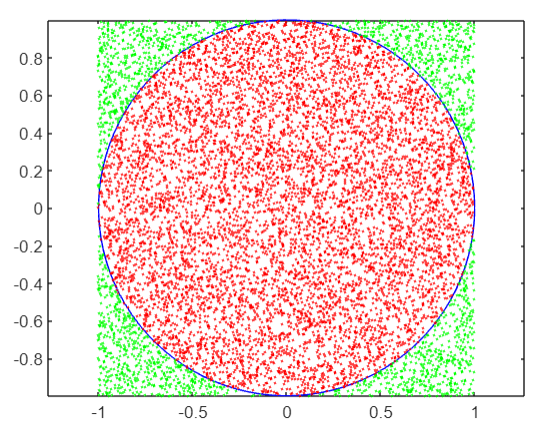
\includegraphics[width=1\textwidth]{graf.png}
        \caption{Naključne točke.}
    \end{figure}
\end{column}
\end{columns}
\end{frame}

\section{Git}

\begin{frame}
\frametitle{GitHub}
\justifying
Nato smo MatLab datoteke in Beamer predstavitev naložili na spletni repozitorij. Na platformi GitHub je nato drug uporabnik izboljšal našo kodo z manjkajočimi oznakami grafa.
\end{frame}

\section{Beamer}

\begin{frame}
\frametitle{Beamer predstavitev}
Predstavitev je morala vsebovati:
\begin{itemize}
    \item Naslovnico, kazalo in logotip fakultete.
    \pause
    \item Tekst in vsaj eno sliko s podnapisom.
    \pause
    \item Funkcijo \textbackslash pause
\end{itemize}
\end{frame}

\end{document}